\section{The Big Picture}
\label{sec:TheBigPicture}
So... what is the Vicon Positioning System? It is a system that captures the drone’s position by using an assortment of Infrared Red (IR) cameras that track reflective IR markers mounted on the drone. The arrangement of cameras inside the flight arena, mounted on the celling, captures the visual feed and is then forwarded to a D-Link switch, which aggregates the camera feeds and sends them onwards to the Vicon Host PC. Inside the Host PC, the Vicon Tracker App computes the compiled visual footage and calculate the UAV’s position, finally broadcasting the positional pose as a continuous string data. \\
\vspace{0.2cm}
There are many ways you can recieve this continuous string of  data from the Host PC. You can either do it wirelesly or wired. For this guide, we will focus on doing this wirelessly via an ethernet port. \\
\vspace{0.2cm}
You will need to setup a Ground Control Station (GCS) that serves as the recieing end of this etherent connection, this is done in a Linux running laptop here. The GCS will reparse the raw positional data recieved into MAVLINK protocol messages, a protocl which majority of drone Flight Controller (FC) uses and understands. Once prased into the correct protocol, we transmit these datas to the drone wirelessly via WiFi. \\
\vspace{0.2cm}
Once the drone recieves this prased positional data, it could be applied for different purposes. In this guide, we will breifly mention how to use this for localisation, path following.
\vspace{0.2cm}
The overall architecture is visualied in \ref{fig:high_level_photo}:

\begin{figure}[H]
    \centering
    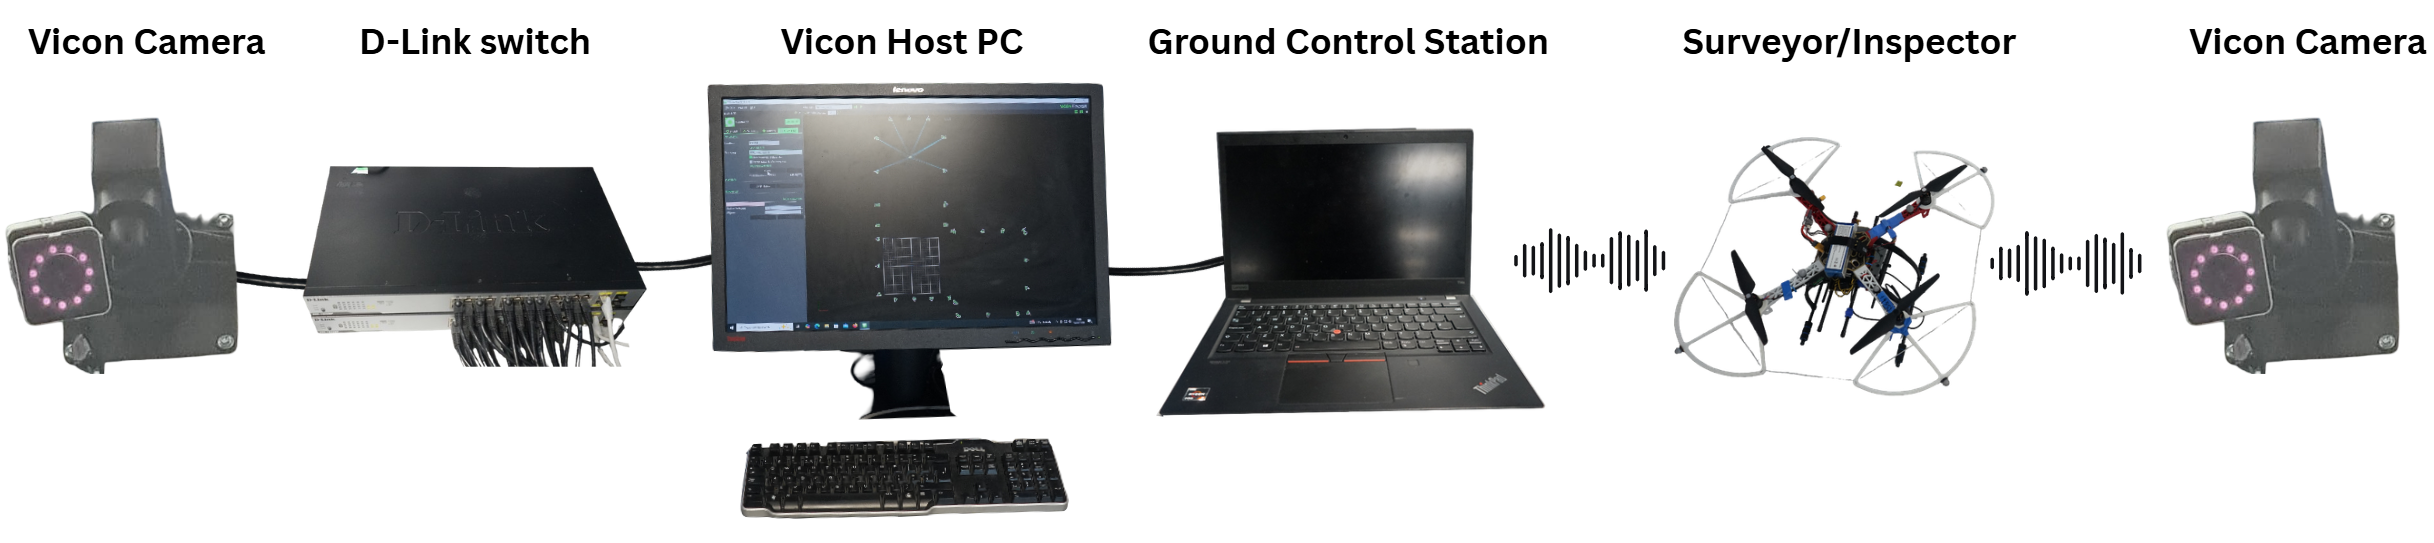
\includegraphics[width=1\linewidth]{Images/Comms Arch.png}
    \caption{A high level flow diagram on the communication for localisation. }
    \label{fig:high_level_photo}
\end{figure}

The wireless telemetry between the GCS and Pixhawk FC uses an ESP8266 WiFi module, jumped directly into the telemetry port of a Pixhawk6C FC, as seen in figure \ref{fig:ground2drone}
 
\begin{figure}[H]
    \centering
    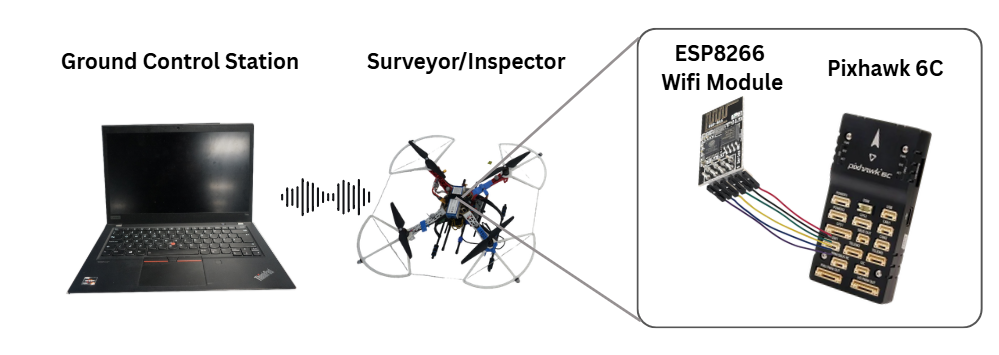
\includegraphics[width=0.8\linewidth]{Images/Ground2Drone.png}
    \caption{Figure on The Wireless Communication Method between GCS and Drone.}
    \label{fig:ground2drone}
\end{figure}

The prasing from raw Vicon data to MAVLink is achieved using a combination of MavProxy (A command line driven Ground Control Station middleware developed by Ardupilot), the Vicon Software Development Kit (SDK) from Vicon, and “PyVicon", a Python3 scirpt written by MathGoron. Together, these software components convert the broadcasted Vicon data into Mavlink in the form of GPS coordinates. This setup is mentioned in great detail in section \ref{sec:GCS}. A figure illustrating the software integration flow as described above is shown below in figure \ref{fig:GCS}:
\begin{figure}[H]
    \centering
    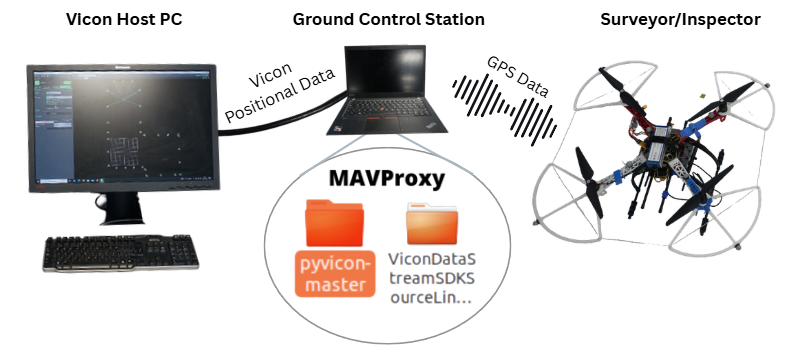
\includegraphics[width=0.8\linewidth]{Images/GCS.png}
    \caption{Figure on the Software Integration in GCS.}
    \label{fig:GCS}
\end{figure}
In the next section in \ref{sec:OperatingVICON}, we will begin the guide with a straight forward procedure on operating the Vicon Positioning System inside the Cranfield Flight Arena. 

\vfill
\begin{center}
    \textbf{This space intentionally left blank}
\end{center}
\vfill

\clearpage